\chapter{\label{app:isc-results}Appendix \textemdash\ Indian subcontinent model results}

% cp /Users/jameswilson/proj/vl_model_isc/figures/dist/isc_logodds.pdf figures/ch5/isc_logodds.pdf

\begin{figure}[tb]
  \centering
  \includegraphics[width=1\textwidth]{figures/ch5/isc_logodds.pdf}
  \caption{Associations between transformed continuous predictors and log(odds) of relapse. For each predictor (excluding parasite grade), a univariable generalised additive model spline fit is shown, with 95\% confidence intervals. For parasite grade, 95\% confidence intervals are calculated for each grade using the Wilson method.}
  \label{fig:isc_logodds}
\end{figure}

\newgeometry{left=1cm, bottom=2.5cm, right=2cm, top=3cm}

% AGE
% cp /Users/jameswilson/proj/vl_model_isc/figures/dist/age_comb.pdf figures/ch5/isc_age_comb.pdf
\begin{landscape}
  \begin{figure}[tb]
    \centering
    \includegraphics[width=1.35\textwidth]{figures/ch5/isc_age_comb.pdf}
    \caption{Distribution of age across studies from the Indian subcontinent. Missing age data described by study.}
    \label{fig:isc_age_comb}
  \end{figure}
\end{landscape}

% HEIGHT
% cp /Users/jameswilson/proj/vl_model_isc/figures/dist/height_comb.pdf figures/ch5/isc_height_comb.pdf
\begin{landscape}
  \begin{figure}[tb]
    \centering
    \includegraphics[width=1.35\textwidth]{figures/ch5/isc_height_comb.pdf}
    \caption{Distribution of height across studies from the Indian subcontinent. Missing data described by study.}
    \label{fig:isc_height_comb}
  \end{figure}
\end{landscape}

% WEIGHT
% cp /Users/jameswilson/proj/vl_model_isc/figures/dist/weight_comb.pdf figures/ch5/isc_weight_comb.pdf
\begin{landscape}
  \begin{figure}[tb]
    \centering
    \includegraphics[width=1.35\textwidth]{figures/ch5/isc_weight_comb.pdf}
    \caption{Distribution of weight across studies from the Indian subcontinent. Missing data described by study.}
    \label{fig:isc_weight_comb}
  \end{figure}
\end{landscape}

% BMI
% cp /Users/jameswilson/proj/vl_model_isc/figures/dist/bmi_comb.pdf figures/ch5/isc_bmi_comb.pdf
\begin{landscape}
  \begin{figure}[tb]
    \centering
    \includegraphics[width=1.35\textwidth]{figures/ch5/isc_bmi_comb.pdf}
    \caption{Distribution of BMI across studies from the Indian subcontinent. Including only participants aged 19 and over (Pandey 2017 excluded). Missing data described by study.}
    \label{fig:isc_bmi_comb}
  \end{figure}
\end{landscape}

% BMI-FOR-AGE Z SCORE
% cp /Users/jameswilson/proj/vl_model_isc/figures/dist/bmiz_comb.pdf figures/ch5/isc_bmiz_comb.pdf
\begin{landscape}
  \begin{figure}[tb]
    \centering
    \includegraphics[width=1.35\textwidth]{figures/ch5/isc_bmiz_comb.pdf}
    \caption{Distribution of BMI-for-age z score across studies from the Indian subcontinent. Including only participants aged from 5--18, inclusive. Missing data described by study.}
    \label{fig:isc_bmiz_comb}
  \end{figure}
\end{landscape}

% WEIGHT-FOR-HEIGHT Z SCORE
% cp /Users/jameswilson/proj/vl_model_isc/figures/dist/wfh_comb.pdf figures/ch5/isc_wfh_comb.pdf
\begin{landscape}
  \begin{figure}[tb]
    \centering
    \includegraphics[width=1.35\textwidth]{figures/ch5/isc_wfh_comb.pdf}
    \caption{Distribution of weight-for-height z score across studies from the Indian subcontinent. Including only participants aged under 5. Missing data described by study.}
    \label{fig:isc_wfh_comb}
  \end{figure}
\end{landscape}

% SPLEEN SIZE
% cp /Users/jameswilson/proj/vl_model_isc/figures/dist/ss_comb.pdf figures/ch5/isc_ss_comb.pdf
\begin{landscape}
  \begin{figure}[tb]
    \centering
    \includegraphics[width=1.35\textwidth]{figures/ch5/isc_ss_comb.pdf}
    \caption{Distribution of spleen size across studies from the Indian subcontinent. Missing data described by study.}
    \label{fig:isc_ss_comb}
  \end{figure}
\end{landscape}

% % FEVER DURATION
% % cp /Users/jameswilson/proj/vl_model_isc/figures/dist/fd_comb.pdf figures/ch5/isc_fd_comb.pdf
% \begin{landscape}
%     \begin{figure}[tb]
%         \centering
%         \includegraphics[width=1.50\textwidth]{figures/ch5/isc_fd_comb.pdf}
%         \caption{Distribution of fever duration across studies from the Indian subcontinent. Missing data described by study.}
%         \label{fig:isc_fd_comb}
%     \end{figure}
% \end{landscape}

% FEVER DURATION LOG SCALE
% cp /Users/jameswilson/proj/vl_model_isc/figures/dist/fd_log_comb.pdf figures/ch5/isc_fd_log_comb.pdf
\begin{landscape}
  \begin{figure}[tb]
    \centering
    \includegraphics[width=1.35\textwidth]{figures/ch5/isc_fd_log_comb.pdf}
    \caption{Distribution of fever duration (log scale) across studies from the Indian subcontinent. Missing data described by study.}
    \label{fig:isc_fd_log_comb}
  \end{figure}
\end{landscape}


% WBC LOG SCALE
% cp /Users/jameswilson/proj/vl_model_isc/figures/dist/wbc_log_comb.pdf figures/ch5/isc_wbc_log_comb.pdf
\begin{landscape}
  \begin{figure}[tb]
    \centering
    \includegraphics[width=1.35\textwidth]{figures/ch5/isc_wbc_log_comb.pdf}
    \caption{Distribution of white blood cell count (log scale) across studies from the Indian subcontinent. Missing data described by study.}
    \label{fig:isc_wbc_log_comb}
  \end{figure}
\end{landscape}

% PLATELETS LOG SCALE
% cp /Users/jameswilson/proj/vl_model_isc/figures/dist/plt_log_comb.pdf figures/ch5/isc_plt_log_comb.pdf

\begin{landscape}
  \begin{figure}[tb]
    \centering
    \includegraphics[width=1.35\textwidth]{figures/ch5/isc_plt_log_comb.pdf}
    \caption{Distribution of platelet count (log scale) across studies from the Indian subcontinent. Missing data described by study.}
    \label{fig:isc_plt_log_comb}
  \end{figure}
\end{landscape}

% HAEMOGLOBIN LOG SCALE
% cp /Users/jameswilson/proj/vl_model_isc/figures/dist/hb_log_comb.pdf figures/ch5/isc_hb_log_comb.pdf

\begin{landscape}
  \begin{figure}[tb]
    \centering
    \includegraphics[width=1.35\textwidth]{figures/ch5/isc_hb_log_comb.pdf}
    \caption{Distribution of haemoglobin (log scale) across studies from the Indian subcontinent. Missing data described by study.}
    \label{fig:isc_hb_log_comb}
  \end{figure}
\end{landscape}

% ALT LOG SCALE
% cp /Users/jameswilson/proj/vl_model_isc/figures/dist/alt_log_comb.pdf figures/ch5/isc_alt_log_comb.pdf

\begin{landscape}
  \begin{figure}[tb]
    \centering
    \includegraphics[width=1.35\textwidth]{figures/ch5/isc_alt_log_comb.pdf}
    \caption{Distribution of alanine transaminase (ALT, log scale) across studies from the Indian subcontinent. Missing data described by study.}
    \label{fig:isc_alt_log_comb}
  \end{figure}
\end{landscape}

% CREATININE LOG SCALE
% cp /Users/jameswilson/proj/vl_model_isc/figures/dist/cr_log_comb.pdf figures/ch5/isc_cr_log_comb.pdf

\begin{landscape}
  \begin{figure}[tb]
    \centering
    \includegraphics[width=1.35\textwidth]{figures/ch5/isc_cr_log_comb.pdf}
    \caption{Distribution of creatinine (log scale) across studies from the Indian subcontinent. Missing data described by study.}
    \label{fig:isc_cr_log_comb}
  \end{figure}
\end{landscape}

\restoregeometry

\newgeometry{left=1cm, bottom=2.5cm, right=1.5cm, top=3cm}

% cp /Users/jameswilson/proj/vl_model_isc/figures/dist/comb_discrete.pdf figures/ch5/isc_comb_discrete.pdf
\begin{landscape}
  \begin{figure}[tb]
    \centering
    \includegraphics[width=1.35\textwidth]{figures/ch5/isc_comb_discrete.pdf}
    \caption{Distribution of categorical predictors by study. Missing data excluded from stacked bar charts for malnutrition, parasite grade. Where aspirates were performed, the source was never missing. NA: unable to show distribution as all study-specific data are missing. MF: miltefosine; SDA: single-dose liposomal amphotericin B}
    \label{fig:isc_comb_dist_cat}
  \end{figure}
\end{landscape}

\restoregeometry

\newgeometry{left=1cm, bottom=2.5cm, right=1.5cm, top=3cm}
%cp /Users/jameswilson/proj/vl_model_isc/figures/dist/ass/cont_cont.pdf figures/ch5/isc_cont_cont.pdf

\begin{landscape}
  \begin{figure}[tb]
    \centering
    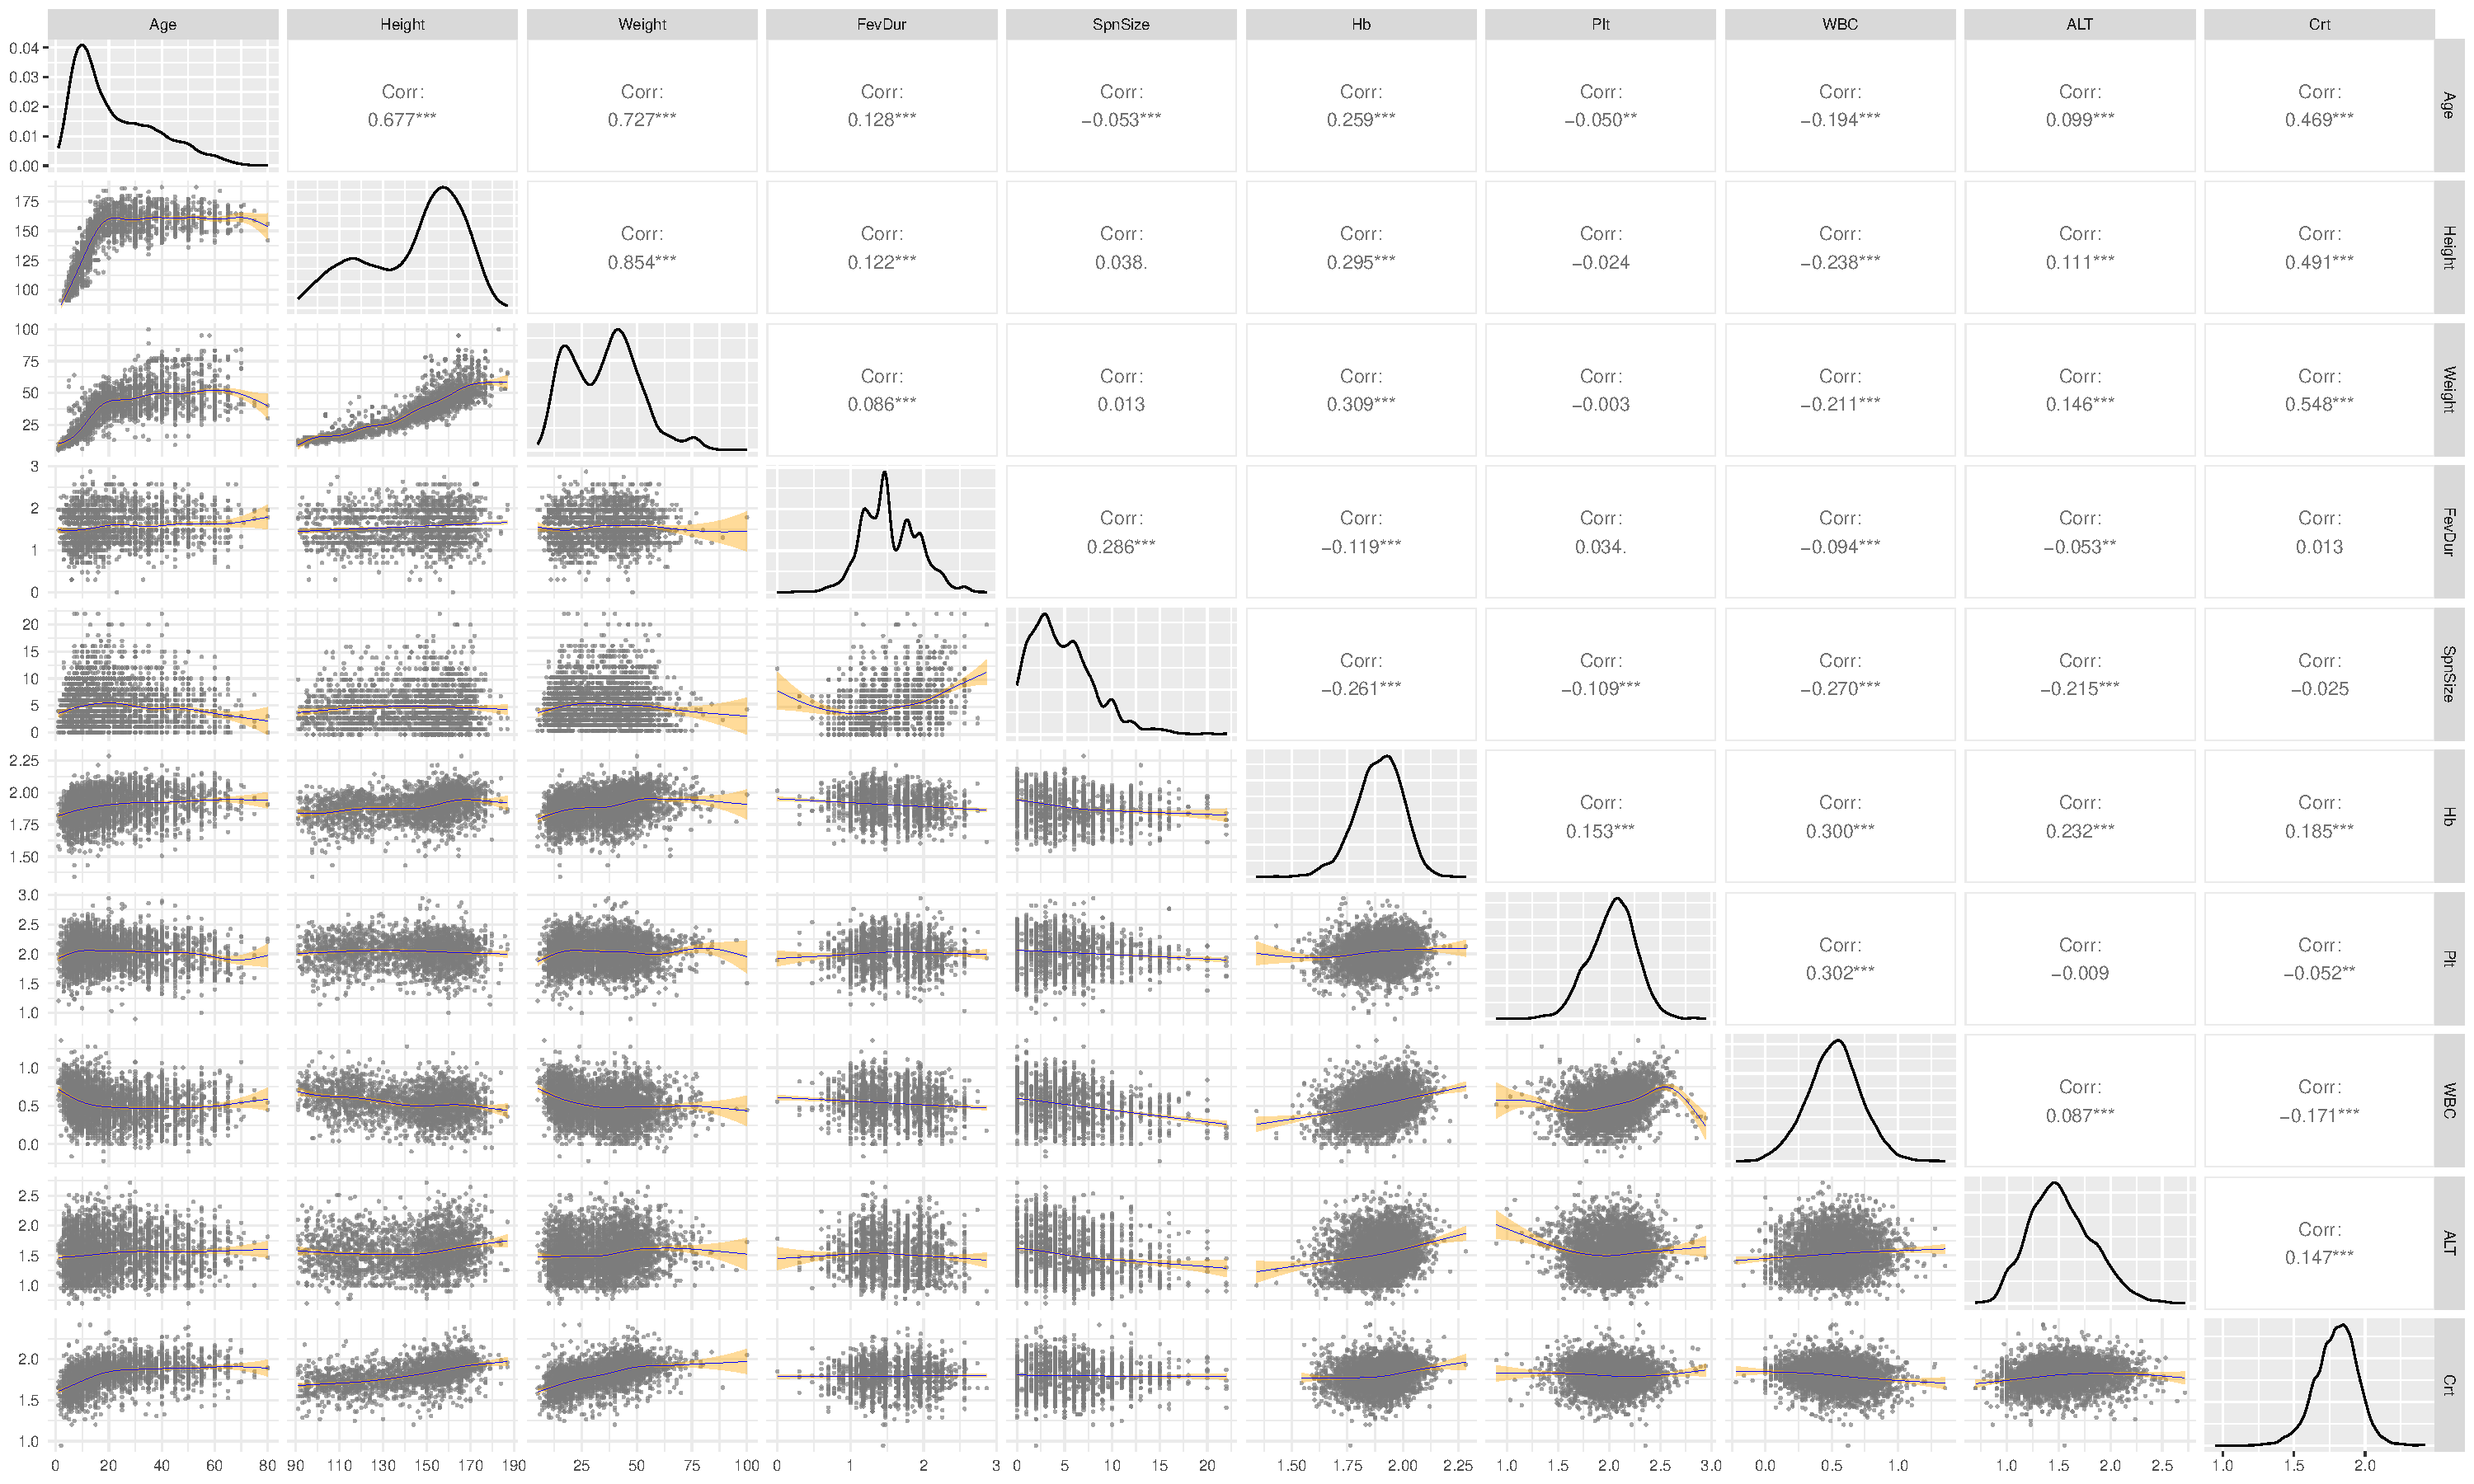
\includegraphics[width=1.34\textwidth]{figures/ch5/isc_cont_cont.pdf}
    \caption{Correlation between continuous variables. For scatter plots, a univariable generalised additive model is fitted (blue line) with 95\% confidence interval ribbon filled (orange area). Pearson correlation coefficients are presented, `***' p<0.001; `**' p<0.01; `*' p<0.05, `.' p<0.10. Age: years; Height: cm; Weight: kg; FevDur: duration of fever, log10(days); SpnSize: spleen size (cm); Hb: haemoglobin, log10(g/L); Plt: platelets, log10($\times10^9/L$); WBC: white blood cells log10($\times10^9/L$); ALT: alanine aminotransferase, log10(U/L); Cr: creatinine log10($\mu$mol/L).}
    \label{fig:isc_cont_cont}
  \end{figure}
\end{landscape}

\restoregeometry

\newgeometry{left=1cm, bottom=2.5cm, right=1.5cm, top=3cm}
%cp /Users/jameswilson/proj/vl_model_isc/figures/dist/ass/cont_cat.pdf figures/ch5/isc_cont_cat.pdf

\begin{landscape}
  \begin{figure}[tb]
    \centering
    \includegraphics[width=1.34\textwidth]{figures/ch5/isc_cont_cat.pdf}
    \caption{Correlation between continuous and categorical variables. FevDur and laboratory tests axes transformed to log10 scale. Age: years; Height: cm; Weight: kg; FevDur: duration of fever, days; SpnSize: spleen size, cm; Hb: haemoglobin, g/L; Plt: platelets, $\times10^9/L$; WBC: white blood cells $\times10^9/L$; ALT: alanine aminotransferase, U/L; Cr: creatinine $\mu$mol/L.}
    \label{fig:isc_cont_cat}
  \end{figure}
\end{landscape}

\restoregeometry

% calibration pots
% cp /Users/jameswilson/proj/vl_model_isc/graphs/calPlotPD.pdf figures/ch5/isc_calPlotPD.pdf
% cp /Users/jameswilson/proj/vl_model_isc/graphs/calPlotFD1.pdf figures/ch5/isc_calPlotFD1.pdf
% cp /Users/jameswilson/proj/vl_model_isc/graphs/calPlotA1.pdf figures/ch5/isc_calPlotA1.pdf
% cp /Users/jameswilson/proj/vl_model_isc/graphs/calPlotAnaemia1.pdf figures/ch5/isc_calPlotAnaemia1.pdf
% cp /Users/jameswilson/proj/vl_model_isc/graphs/calPlotRx1.pdf figures/ch5/isc_calPlotRx1.pdf

\begin{figure}[tb]
  \centering
  \includegraphics[width=0.8\textwidth]{figures/ch5/isc_calPlotPD.pdf}
  \caption{Calibration plots for parasite grades \textemdash\ model including parasite grade.}
  \label{fig:isc_calPlotPD_ap}
\end{figure}

\begin{figure}[tb]
  \centering
  \includegraphics[width=0.8\textwidth]{figures/ch5/isc_calPlotFD1.pdf}
  \caption{Calibration plots for fever duration \textemdash\ model including parasite grade.}
  \label{fig:isc_calPlotFD1_ap}
\end{figure}

\begin{figure}[tb]
  \centering
  \includegraphics[width=0.8\textwidth]{figures/ch5/isc_calPlotA1.pdf}
  \caption{Calibration plots for age \textemdash\ model including parasite grade.}
  \label{fig:isc_calPlotA1_ap}
\end{figure}

\begin{figure}[tb]
  \centering
  \includegraphics[width=0.8\textwidth]{figures/ch5/isc_calPlotAnaemia1.pdf}
  \caption{Calibration plots for anaemia severity \textemdash\ model including parasite grade.}
  \label{fig:isc_calPlotAnaemia1_ap}
\end{figure}

\begin{figure}[tb]
  \centering
  \includegraphics[width=0.8\textwidth]{figures/ch5/isc_calPlotRx1.pdf}
  \caption{Calibration plots for treatment \textemdash\ model including parasite grade.}
  \label{fig:isc_calPlotRx1_ap}
\end{figure}


% model without parasite grade

\begin{figure}[tb]
  \centering
  \includegraphics[width=0.8\textwidth]{figures/ch5/isc_calPlotFD2.pdf}
  \caption{Calibration plots for fever duration \textemdash\ model \textbf{not} including parasite grade.}
  \label{fig:isc_calPlotFD2_ap}
\end{figure}

\begin{figure}[tb]
  \centering
  \includegraphics[width=0.8\textwidth]{figures/ch5/isc_calPlotA2.pdf}
  \caption{Calibration plots for age \textemdash\ model \textbf{not} including parasite grade.}
  \label{fig:isc_calPlotA2_ap}
\end{figure}

\begin{figure}[tb]
  \centering
  \includegraphics[width=0.8\textwidth]{figures/ch5/isc_calPlotAnaemia2.pdf}
  \caption{Calibration plots for anaemia severity \textemdash\ model \textbf{not} including parasite grade.}
  \label{fig:isc_calPlotAnaemia2_ap}
\end{figure}

\begin{figure}[tb]
  \centering
  \includegraphics[width=0.8\textwidth]{figures/ch5/isc_calPlotRx2.pdf}
  \caption{Calibration plots for treatment \textemdash\ model \textbf{not} including parasite grade.}
  \label{fig:isc_calPlotRx2_ap}
\end{figure}

% cp /Users/jameswilson/proj/vl_model_isc/graphs/forestCIM2.pdf figures/ch5/forestCIM2.pdf
% forest plots for C-statistic - WITHOUT PARASITE GRADE
\begin{figure}[tb]
  \centering
  \begin{overpic}[width=0.9\textwidth, trim={3.5cm 0cm 1cm 0.3cm}, clip]{figures/ch5/forestCIM2.pdf}
    \put(0,5.5){\scriptsize $\tau^2$: 0.62; $I^2$: 82.8\%}
    \put(0,2.3){\scriptsize Q(df = 17): 134.88; p < .0001}
  \end{overpic}
  \caption{Forest plot showing individual and pooled study c--statistics, for the model \textbf{excluding} parasite grade. Pooled c--statistics are presented from both fixed--effects and random--effects meta-analysis models. Pooled random--effects c--statistics and variances are estimated using restricted maximum likelihood (REML) and the Hartung--Knapp--Sidik--Jonkman method. Blue diamonds: pooled summary estimates with 95\% confidence intervals. Red line: 95\% prediction interval. Study ordered by c--statistic. For Chakraborty 2008, no relapse events occurred and c--statistic is therefore undefined. Study--specific confidence intervals should be interpreted with caution due to small sample sizes and relapse events in some studies (see Methodology Section \ref{meth:discrimination}).}
  \label{fig:isc_forestCIM2}
\end{figure}

% cp /Users/jameswilson/proj/vl_model_isc/graphs/forestCalM2.pdf figures/ch5/forestCalM2.pdf
% forest plots for calibration
\begin{figure}[tb]
  \centering
  \begin{overpic}[width=0.9\textwidth, trim={3.4cm 0cm 0.3cm 0.3cm}, clip]{figures/ch5/forestCalM2.pdf}
    \put(27,13){\fcolorbox{black}{white}{\tiny $\tau^2$: 0.14; $I^2$: 55.8\%; Q(17): 39.5; p = .0015}}
    \put(68,13){\fcolorbox{black}{white}{\tiny $\tau^2$: 0.006; $I^2$: 1.32\%; Q(16): 14.7; p = .62}}
  \end{overpic}
  \caption{Forest plots showing individual and pooled study calibration measures, for the model \textbf{excluding} parasite grade. Left: calibration intercept (calibration--in--the--large); Right: calibration slope. Pooled summary estimates and variances are estimated from random--effects meta-analysis models using restricted maximum likelihood (REML) and the Hartung--Knapp--Sidik--Jonkman method. Blue diamonds: summary estimates with 95\% confidence intervals. Red lines: 95\% prediction interval. Calibration measures not presented for Chakraborty 2008 due to no relapse events. Calibration slope not presented for Rijal 2010(A) due to only one relapse event and few total participants leading to failure of model convergence.}
  \label{fig:isc_forestCalM2}
\end{figure}